\documentclass[conference]{IEEEtran}
\IEEEoverridecommandlockouts
% The preceding line is only needed to identify funding in the first footnote. If that is unneeded, please comment it out.
\usepackage{cite}
\usepackage{amsmath,amssymb,amsfonts}
\usepackage{algorithmic}
\usepackage{graphicx}
\usepackage{textcomp}
\usepackage{xcolor}
\def\BibTeX{{\rm B\kern-.05em{\sc i\kern-.025em b}\kern-.08em
    T\kern-.1667em\lower.7ex\hbox{E}\kern-.125emX}}
    
    
%To include Assamese Text in the paper(Execute The file in XeTex)
\usepackage{fontspec}
\usepackage{polyglossia}
\setmainlanguage{english}
\setotherlanguages{bengali}
\newfontfamily\bengalifont[Script=Bengali]{Lohit Assamese}



\begin{document}

\title{Assamese VADER: A Sentiment Analysis Approach Using Modified VADER\\
}

\author{\IEEEauthorblockN{Chandana Dev}
\IEEEauthorblockA{\textit{Assam Engineering College}\\
Guwahati,India \\
chandanaaec@gmail.com}
\and
\IEEEauthorblockN{Dr. Amrita Ganguly}
\IEEEauthorblockA{\textit{Assam Engineering College}\\
Guwahati, India \\
aganguly.ele@aec.ac.in}
\and
\IEEEauthorblockN{Hsuvas Borkakoty}
\IEEEauthorblockA{\textit{Tezpur University}\\
Tezpur, India \\
hsuvas@tezu.ernet.in}

}

\maketitle

\begin{abstract}
Sentiment Analysis is a Natural Language Processing (NLP) technique that determines the opinion towards an entity, identifying the opinion as positive, negative, or neutral. Extensive research has taken place for high-resourced Languages like English, whereas for Low resourced Indo-Aryan languages, it is still an area in progress. This paper attempts to perform Sentiment Analysis on Assamese Texts, which is a morphologically rich yet Low-resource Indo-Aryan Language, using the concepts of popular sentiment analyzer named ``Vader”, while taking ``Bengali-Vader” as its backbone. The process follows that of a traditional Vader tool, with consideration towards creating a dictionary of negative booster words and creating an Assamese Lexicon, pre-processing of data, boosting the valence of each word, valence calculation and sentiment categorization of text based on the valence. The necessity of proper dataset in this method is immense, and even though the lack of good translation tools and resources to feed the model, this model was experimented on a set of Assamese texts from a renowned Assamese novel. The comparison was done by manually translating the Assamese sentences to its Bengali and English forms and it shows significant results when compared with the Bengali and English counterparts.
\end{abstract}

\begin{IEEEkeywords}
Sentiment Analysis, Natural Language Processing, Vader, Assamese.
\end{IEEEkeywords}

\section{Introduction}
Sentiment analysis is a technique to identify the emotions towards an entity. It can be of different types viz positive, negative or neutral. Sentiment analysis refers to the feature extraction of one‘s emotions towards an entity. Researchers from various fields are using computational techniques on different entities like Audio, Video, Images, and Texts etc. to perform sentiment analysis. With enormous data generating everyday on web, social media etc. sentiment analysis and its applications has become a highly interesting topic to NLP researchers.

Sentiment analysis on textual data is no longer restricted to one or two languages. Data scientists of this research area have moved into multiple languages used across the globe. With rapid growth of textual data on multiple languages sentiment analysis in multilingual data has opened a new research window to NLP engineers. Amongst various international languages like English, French, German, etc many Indian language has been able to establish their existences in the field of NLP research since last few couple of years. Bengali, Tamil, Oria, Kannada, Hindi etc being few of them.Assamese language, which is a morphologically rich Indo-Aryan language mostly spoken mainly in the north eastern state of India, especially in Assam, where it is an official language, with around 14 million speakers [1]. Very limited research work has been performed on the same even though it is being one of the socially and culturally enriched languages of North-eastern India. In terms of social and cultural aspect many works have been performed in this language since many hundred years. But at the same time in terms of computational aspects it has been still in the stage of
almost unexplored for NLP engineers. Due to very limited available resources in terms of datasets Assamese language is still in such level of research. Sentiment analysis on this language is not yet being explored by data scientists. In this paper works have been done in this direction. Bengali being the sister language of Assamese ~\cite{b1} has enormous morphological analogy to Assamese. In this paper we have used Bengali VADER ~\cite{b2} modified from popular English sentiment classification tool VADER ~\cite{b3} and upgraded it to support Assamese sentiment analysis without using any Assamese to English translation.

Following sections discussed the various aspects of our work for developing the sentiment analysis tool.

Section II describes about the literature review of NLP tasks performed on Assamese language. Section III describes briefly about the English VADER tool. In section IV we discuss about our approach to develop VADER tool in Assamese language from English Lexicon. In section III we have also discussed about our methodology and proposed Assamese VADER. Finally Section IV describes about the results and discussion followed by our conclusion of the work in section V with all the possible future aspects.

\section{Literature Review}

\subsection{Lexicon}

Dictionary meaning of a lexicon is the complete set of meaningful units in a language. Polarity lexicons are that which have a listing of words with initial level of polarities. It is one of the important resources for sentiment analysis in texts using computational techniques. There are primarily three ways to build polarity lexicons: interpreting existing lexicons from different languages, extracting polarity lexicons from corpora ~\cite{b4}, and annotating sentiments Lexical Knowledge Base~\cite{b5}~\cite{b6}~\cite{b7}~\cite{b8}.Four major languages there are well known manually constructed lexicons such as General Inquirer ~\cite{b9}, Opinion Finder ~\cite{b10}, SO-CAL ~\cite{b11}, etc. In ~\cite{b12} and ~\cite{b13}authors analyzed the methodology of translating English resources to Romanian and Spanish respectively. There are several English polarity lexicons available online such as SentiWordNet, VADER but hardly any Assamese polarity lexicon.

\subsection{English Language}

Enormous works on sentiment analysis in English language have been performed such as VADER. In this model, researchers combined qualitative and quantitative methods to produce a gold- standard sentiment lexicon, which was later empirically validated against especially receptive micro blog type contexts. VADER combines important lexical features obtained from five generalized rules that embody grammatical and syntactical conventions of human speech. It also retains the advantages of conventional sentiment lexicons such as LIWC ~\cite{b14}~\cite{b15}.

In ~\cite{b8} authors explored three strategies to build polarity lexicons: interpreting existing lexicons from other languages, explaining sentiments from lexical knowledge bases and extracting polarity lexicons from corpora. All of the models require different degrees of human effort. Here Spanish lexicon ~\cite{b16} has been translated by means of the Elhuyar Spanish dictionary, where Spanish word incorporates five interpretations.

\subsection{VADER}

VADER is a simple rule based for general sentiment analysis developed by comparing its effectiveness to eleven typical states of practice benchmarks. VADER tool has produced a gold-standard sentiment lexicon by combining qualitative and quantitative methods. This tool works exceptionally well in social media. Sentiment analysis models work significantly on good sentiment lexicons. Sentiment lexicon is a list of words which are commonly classified as per their semantic orientations such as positive or negative ~\cite{b17}.Once the lexicon is built and validated; it is then used to evaluate the sentiments of the texts. Following framework shows the built up of VADER-English model:
\begin{enumerate}
    \item Data Preprocessing: This step involves
            \begin {itemize}
            \item Tokenization: By this text datas are converted into tokens.
            \item Stop words removal: By this words without any sentiments like is, are, of, from etc are removed from the texts.
            \item Punctuation removal: Here punctuations bearing no sentiments are cleaned from the input data.
            \end{itemize}
    \item Data Boosting :Once the data pre-processing is performed each cleaned tokens are the checked for valence boosting purpose. Boosting data are those which have terms like ‘very’, ’great’, ’extremely’ etc. If such words are found in the text the valance of the word is boosted .Texts are then checked for idioms phrases followed by ‘but’ words search. In both the cases valence of the words are further boosted.
    \item Valence Calculation: In this step valence of a sentence is calculated which lies between -4 to +4 ~\cite{b3}.This calculation is further normalized to range -1 to +1.Thus each and every sentence of the whole documents/dataset are assigned with respective sentiment polarity. 
\end{enumerate}

\subsection {Assamese Language}
Sentiment analysis in Bengali language has reached almost equal milestones in comparison to English language. NLP tasks in this language have already been explored in many dimensions. But being sister language to Bengali, Assamese language have still been almost unexplored one in the same field of research. In terms of dataset, researchers have a very easy excess of Bengali language as Google translator is incorporated with the same. Whereas this kind of accessibility is unavailable in Assamese language. Very few datasets which can be considered as negligible are actually available to do any primitive to advanced levels of NLP tasks in Assamese language. There is not even any sentiment lexicon like SentiwordNet which is available in various Indian languages like Hindi, Bengali, and Nepali etc. The authors of ~\cite{b18} have translated the SentiWordNet in Bengali and used its polarity to calculate the valence of Bengali texts.

\section{Proposed Assamese Vader}
We have developed a model to identify sentiments from Assamese texts. We have performed sentence level sentiment analysis. In our work we had to prepare lexicon manually by translating Bengali lexicon to Assamese, which was initially translated from Google translators for development of Bengali VADER. Manual translation of word by word was in fact a very tedious work to perform .Hence we had to limit our translation to 500 words only from the available lexicon used in English Vader.

Following steps are followed while creating the tool for Assamese VADER.

\begin{enumerate}
    \item  Dictionary creation: Two dictionaries - Negation words and Booster words have been developed. Negation words dictionary consists of those words which are commonly used in Assamese language to represent the negative sense of the texts. Any sentence having such words will be reversed in polarity to either positive or to negative. Some examples are 
    \begin{bengali}
    ‘ন’ , ‘নাই’, ‘নকৰিব’, ‘নকৰো’, ‘নকৰিলে’, ‘নলয়’, ‘নহলে’, ‘ নহব’ , ‘নাই হোৱা’ , ‘নাইকৰা’, ‘নাই লোৱা’ , ‘কৰা নাই’, ‘হোৱা নাই’,  ‘ভাল নহয়’,  ‘বেয়া নহয়’,  ‘নহয়’,  ‘নহলে’ , ‘নহবলগীয়া’.
    \end{bengali}

    Booster dictionary consists of words that are used to boost valence of any texts are included. If any such words are present in the texts then polarity of the texts are increased in our model.  Such words are
    \begin{bengali}
    ‘বেছি’, ‘খুব’, ‘বহুত’, ‘অতি’, ‘অধিক’, ‘অত্যাধিক’
    \end{bengali}etc.

    \item Assamese lexicon: Manual translations have been done for about 500 words taken from English Vader lexicon which is originally translated to Bengali by using Google translator. Since manual translation is a tedious work to perform hence to test our model we have chosen to use 500 words from the same. Human translator has helped us in this context. Polarity of each word has been kept same as given in original English Vader lexicon. The valence of the words is kept in the range of -4 to +4. Where -4 represent most negativity, +4 represent most positivity and ‘0’ represents neutral sentiments.
    
    \item Pre-processing of data:
            \begin{itemize}
                \item Tokenization: In this step punctuation as well as stop words has been removed from the texts whose sentiments need to be evaluated. For e.g the following text: সি খুব ভাল নহয় – ‘He is not that good’ will appear as - \begin{bengali} ‘সি’ , ‘খুব’,  ‘ভাল’,  ‘নহয়’ \end{bengali} after tokenization. After punctuation removal it will appear as same as above. 
                
                \item Assamese stopwords removal: Words which do not have any sentiments are called stop-words. We have created list of Assamese stop words as they are not easily available in web. Such words are – \begin{bengali}‘সি’, ‘মোৰ’, ‘মই’, ‘তেওঁ’, ‘আৰু’, \end{bengali} etc i.e ‘he/she’, ‘I’, ‘me’, ‘and’ etc. When such words are found in the sentence token list, they are removed. Hence for previous example \begin{bengali} সি  খুব  ভাল  নহয় \end{bengali}.Ater stop words removal tokens will appear as \begin{bengali} ‘খুব’, ‘ভাল’, ‘নহয়’.\end{bengali}
                
                \item Stemming: Stemming in natural language processing is a method to reduce any type of derived words into their original word or ‘stem’. In case Assamese Vader model, we have performed stemming words to its root words so that the same can be easily compared to the lexicon. First we have verified the requirement of the word for stemming. Words having \begin{bengali}‘ৰ’, ‘টো’,‘ডাল’, ‘খন’ \end{bengali} etc at the end are stemmed. Stemming is then followed by negation check list in the texts. At this stage we check \begin{bengali}‘নহয়’, ‘নহব’, ‘নাই’\end{bengali} etc at the end of the word. Example of stemming: \begin{bengali}‘বিপদৰ সময়ত নহয়’\end{bengali} –not in the time of danger will appear as \begin{bengali} ‘বিপদ’, ‘সময়’, ‘নহয়’\end{bengali}.After negation check it will appear as \begin{bengali} ‘বিপদ’, ‘সময়’, ‘ন’, ‘হয়’.\end{bengali}
                
                \item Boosting word valence: Here boosting words are searched I the texts .When such words are found in the text, valance of the same is intensified according to the position of the booster word in the sentence position checking of the boost- er words have been done by ‘bigram’, trigram’, method. In bigram method two adjacent tokens are searched. In trigram method three adjacent tokens are searched. For any word when found in booster dictionary, in bigram tokens valence of the word is multiplied by 0.9 and for trigram tokens it is multiplied by 0.75 ~\cite{b3}. Presence of negation words are generally affects the overall sentiments of the sentence. But in Assamese language negation words are differently used as compared to English text. In Assamese texts these words are used generally at the end of the sentence where as in English they are used in the middle of the texts. Negation words are searched as per the list of words included in the negation words list which is constructed in the beginning. Valence of the sentence is multiplied by -1 i.e. reverse of the existing valence of the sentence.

                \item Calculation of valence: Our model helps to find the valence of text accurately .This model is built to output sentiment polarity as positive, negative and neutral. But is further re- quires normalization.
                 \begin{equation}
                     Normalized Score =\frac{score}{\sqrt{score^2 + \alpha}}
                 \end{equation}
                Where $\alpha$ =15 is approximated maximum expected value and score is calculated score to be normalized.
                
                \item Sentence separation: Sentence is categorized as neutral, negative, positive as per polarity calculated from the valence of texts between -1 to 0, then it is negatively expressed sentence. Here ‘0’ represents neutral sentiment of the sentence, when the valence range lies in between 0 to +1, then it is considered as positively expressed sentence.
            \end{itemize}
            
\end{enumerate}
The step by step procedure is depicted in Figure \ref{fig:proc}.
\begin{figure}[htbp]
    \begin{center}
        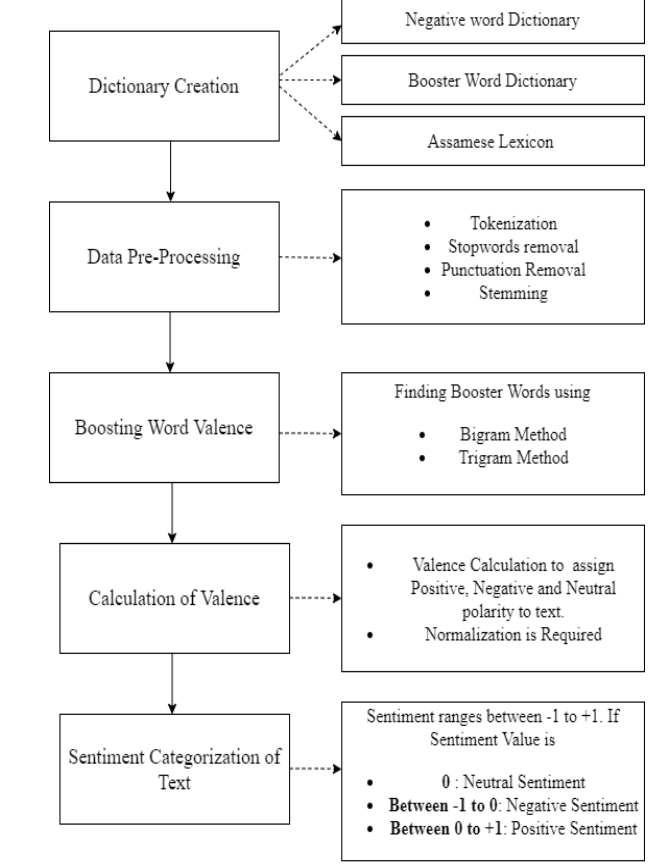
\includegraphics[width=2in]{proc.png}
        \caption{Flow diagram of Methodology}
        \label{fig:proc}
    \end{center}
\end{figure}

\section{Results and Discussion}

Initially some sample sentences have been taken which are randomly chosen and then the sample sentences have been analyzed with the modeled Vader tool where the results were satisfactory in terms of human standard, that is, the results match with human sentiments. The experiment is continued by providing excerpts of an Assamese famous novel. The results of some of the sentences that are achieved have been compared with Bangla VADER ~\cite{b2} and English VADER ~\cite{b3} where the translations of the sentences are done manually. The comparison of results is being shown in the Table ~\ref{tab1}. The table also contains the human sentiment extracted manually. Since Human sentiments are absolute in nature, therefore -1, 0 and 1 is as- signed for Negative, Neutral and Positive sentiments respectively. The novel contains most of neutral sentiments sentences, thus the experiment also have shown same sentiments after performing the analysis.


\begin{table}[htbp]
    \caption{Sentiment comparison of Different Vader tools(Including Human Sentiment}
    %\begin{center}
    \resizebox{.5\textwidth}{!}{ %
    \begin{tabular}{|c|c|c|c|c|c|}
    \hline
    \textbf{Serial No.} &\textbf{Sentences}&\textbf{Assamese Score}&\textbf{Bengali Score}&\textbf{English Score}&\textbf{Human Score} \\
     \hline
    1 & \begin{bengali}সি খুব বেয়া নহয় ।\end{bengali} (He is not so bad) & 0 & 0.659 & 0.4708 & 0 \\
      \hline
    2 &  \begin{bengali}মই মোৰ মতে ভালে আছো।\end{bengali}  (I am fine in my opinion) & 0.4404 & 0.6597 & 0.2732 & 1 \\
      \hline
    3 & \begin{bengali}ব্যৰ্থতা সাফল্যৰ চাবি।\end{bengali}  (Failure is the key to success) & 0 & 0.1027 &0.1027 & 0 \\
      \hline
    4 &  \begin{bengali}নিজৰ ওপৰত আত্নবিশ্বাস থকা ভাল।\end{bengali} (It is good to have self-confidence) & 0 & 0.7096 & 0.6908 &0 \\
      \hline
    5 & \begin{bengali} তেওঁ এজন আদৰ্শ শিক্ষক। \end{bengali} (He is an ideal teacher) & 0 & 0.5267 & 0.5267 & 1 \\
      \hline
    6 & \begin{bengali} সি ভুত ভয় কৰে। \end{bengali} (He is afraid of ghosts) & -0.4019 & 0.7003 & 0.0 & -1 \\
      \hline
    7 & \begin{bengali} মোৰ সৌভাগ্য হোৱা নাই।\end{bengali} (I have not been  fortunate) & -0.3818 & -0.3818 & -0.3412 & -1 \\
      \hline
    8 & \begin{bengali}সি পৰিশ্ৰমী নহয়। \end{bengali} (He is not hardworking) & 0 & -4767 & 0.0 & -1 \\
      \hline
    9 & \begin{bengali}কি ধুনীয়া খৱৰ। \end{bengali} (What a good news!) & 0 & 0.4767 & 0.5994 & 1 \\
      \hline
    10 & \begin{bengali} ফান্দত ভৰি নিদিব।\end{bengali} (Don't put your foot in the trap) & 0 & 0.3182 & -0.3182 & 0 \\
      \hline
    11 & \begin{bengali}সি পঢ়াত মনোযোগী নহয়।\end{bengali} (He is not attentive towards studies) & 0 & 0.-3818 & 0 & -1 \\
      \hline
    12 & \begin{bengali} বুদ্ধিমানৰ লগত লাগি থাকিলে আপুনিও সফল হব।\end{bengali} (If you stay with intelligent people, you will be successful.) & 0.4215 &  0.7003 & 0.6486 & 1 \\
      \hline
    13 & \begin{bengali} মই মোৰ মাক বহুত ভাল পাও।\end{bengali} (I love my mother a lot) & 0.4927 & 0.6697 & 0.6369 & 1 \\
      \hline
    14 & \begin {bengali} সি খুব বেছি ভয় কৰা নাই। \end{bengali} (He is not much afraid) & 0.4576  & 0.5034 & 0.6369 & 1 \\
      \hline
    15 & \begin{bengali} উজ্জ্বল বস্তু মাত্ৰেই সোন নহয়।\end{bengali}(Not everything that shines is gold) & -0.4404 & 0 & 0.4404 & -1 \\
      \hline
    16 & \begin{bengali} এখন কঁপি থকা ৰামধেনু। \end{bengali} (A tremating rainbow) & 0 & 0 & 0 & 0 \\
      \hline
    17 & \begin{bengali} উদ্দেশ্য নাই, চিন্তা নাই, ভাবনা নাই। \end{bengali} (No purpose, no worries, no thought.) & 0.4404 & 0.4404 & 0 & 0 \\
    \hline
\end{tabular}
}
\label{tab1}
%\end{center}
\end{table}


With all the methodologies mentioned in the previous sections, results have been achieved where it shows whether the sentence is positive, negative or neutral. Evaluation of results has also been done with VADER tool which is built with English /Bengali language. For evaluation, Assamese texts have been translated to English manually and then sentiment polarity has been compared. The noteworthy point here is the affect of the lack of resources in calculation of sentiments. The comparison of the tool is done with English VADER, which contain 7062 lexicons, whereas for Assamese VADER, we were manually able to translate 300 Lexicons. This provides a difference in results for the same sentence. For example, in the sentence \begin{bengali} সি খুব বেছি ভয় কৰা নাই।\end{bengali} (Translation:   He is not much afraid), the sentiment scores are 0.4576 from Assamese VADER, 0.5034 from Bengali VADER and 0.3412 from English Vader. The human sentiment detection classifies it as Positive, which is same as the result from all the VADER tools. Although the lack of Assamese lexicons show difference in results, the sentiment polarity remains unchanged in almost all cases. The above example shows the justification for the said statement. This implies that improvement scope in performance of this experiment is tremendous if one can translate the whole Vader lexicon of English.

A graphical representation of the scores is also given in Figure
~\ref{fig:bar1}. The figure depicts a bar chart of the sentiment scores of the statements in three languages, Assamese, Bengali and English.

\begin{figure}[htbp]
    \begin{center}
        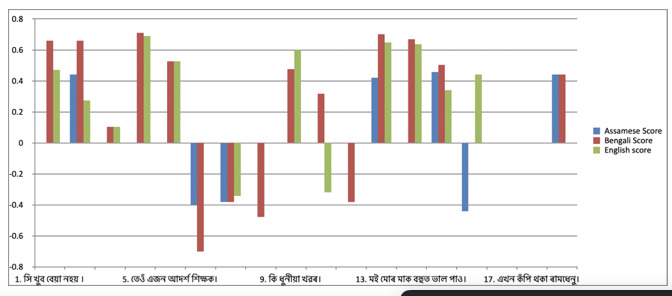
\includegraphics[height=2in,width=3in]{bar1.png}
        \caption{Bar chart of Comparison of Sentiment Scores in Assamese,English and Bengali Vader}
        \label{fig:bar1}
    \end{center}
\end{figure}

The color code for the respective languages are Blue, Red and light Green, for Assamese, Bengali and English respectively. It is shown in the figure that the difference of values in all the three languages, and it can be said that even though the lack of lexicon shows certain difference in measurement of polarity, our Assamese VADER provides a satisfactory results, despite of the hurdles.

Another interesting representation of the result is depicted in Figure ~\ref{fig:bar2}. The comparison of human sentiment for a set of par- ticular sentences from Table 1 and same in our Assamese VADER tool has been done in Figure ~\ref{fig:bar2} through a bar graph.
\begin{figure}[htbp]
    \begin{center}
        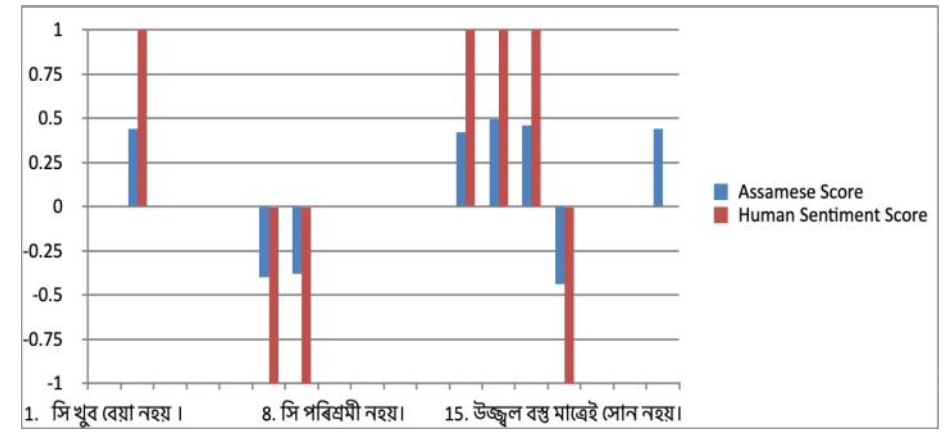
\includegraphics[height=2in,width=3in]{bar2.png}
        \caption{Bar chart of Comparison of Sentiment Scores in Assamese,English and Bengali Vader}
        \label{fig:bar2}
    \end{center}
\end{figure}

As evident from the Figure, the Score of Assamese VADER and Human Sentiment Score that have been obtained manually shows similar sentiment scores. However, the scenario depicted here is with a limited lexicon for the tool only, that is, some deviation might be obtained when the input size grows. This can be overcome through growing the lexicon of the VADER tool, which also can improve performance drastically.

\section{Conclusion}
In this paper we have presented the development of Assamese VADER by modifying the existing English VADER taking Bengali VADER as backbone. The existing English VADER has been modified to detect the sentiment polarity of Assamese texts using Assamese Lexicon. In the process we have used boosting words, apply bigram, trigram to test the system in order to have better performance of the model. From the experimental analysis we have observed that our proposed model works efficiently on Assamese texts. With the unavailability of resources in Assamese language it was very difficult initially to test the model with minimum data. With the increase of data size i.e by increasing the manual translated words of Assamese texts used in the lexicon, performance has been improved. In future we aim to translate whole Vader lexicon of English and build a machine learning algorithm to design a classifier so that the existing model performance can be compared in terms of efficiency.







\begin{thebibliography}{00}
\bibitem{b1} "Abstract of Speakers' Strength of Languages and Mother Tongues - 2011" (PDF). censusindia.gov.in. Retrieved 15 February 2021.

\bibitem{b2} Al Amin, Imran Hossain, Aysha Akther* and Kazi Masudul Alam, ―Bengali VADER: A Sentiment Analysis Approach Using Modified VADER,‖ in International Conference on Electrical, Computer and Communication Engineering (ECCE), 7-9 February, 2019.

\bibitem{b3} C. H. E. Gilbert, ―Vader: A parsimonious rule-based model for sentiment analysis of social media text,‖ in Eighth International Conference on Weblogs and Social Media (ICWSM-14). Available at (20/04/16) http://comp. social. gatech. Edu/papers/icwsm14. vader. hutto. pdf, 2014.

\bibitem{b4} V. Hatzivassiloglou and K. R. McKeown, ―Predicting the semantic orientation of adjectives,‖ in Proceedings of the 35th annual meeting of the association for computational linguistics and eighth conference of the european chapter of the association for computational linguistics. Association for Computational Linguistics, 1997, pp. 174–181.

\bibitem{b5} S.-M. Kim and E. Hovy, ―Determining the sentiment of opinions,‖ in Proceedings of the 20th international conference on Computational Linguistics. Association for Computational Linguistics, 2004, p. 1367.

\bibitem{b6} J. Kamps, M. Marx, R. J. Mokken, M. De Rijke et al., ―Using wordnet to measure semantic orientations of adjectives.‖ in LREC, vol. 4. Citeseer, 2004, pp. 1115–1118.

\bibitem{b7} H. Liu and P. Singh, ―Concept net—a practical common sense reasoning tool-kit,‖ BT technology journal, vol. 22, no. 4, pp. 211–226, 2004.

\bibitem{b8} I. San Vicente and X. Saralegi, ―Polarity lexicon building: to what extent is the manual effort worth?‖ in LREC, 2016.

\bibitem{b9}  P. J. Stone, D. C. Dunphy, and M. S. Smith, ―The general inquirer: A computer approach to content analysis.‖ 1966.

\bibitem{b10}  T. Wilson, P. Hoffmann, S. Somasundaran, J. Kessler, J. Wiebe, Y. Choi, C. Cardie, E. Riloff, and S. Patwardhan, ―Opinion finder: A system for subjectivity analysis,‖ in Proceedings of hlt/emnlp on interactive demonstrations. Association for Computational Linguistics, 2005, pp. 34–35.

\bibitem{b11} M. Taboada, J. Brooke, M. Tofiloski, K. Voll, and M. Stede, ―Lexicon based methods for sentiment analysis,‖ Computational linguistics, vol. 37, no. 2, pp. 267–307, 2011.

\bibitem{b12}R. Mihalcea, C. Banea, and J. Wiebe, ―Learning multilingual subjective language via cross-lingual projections,‖ in Proceedings of the 45th annual meeting of the association of computational linguistics, 2007, pp. 976–983.

\bibitem{b13} V. Perez-Rosas, C. Banea, and R. Mihalcea, ―Learning sentiment lexicons in spanish.‖ in LREC, vol. 12, 2012, p. 73.

\bibitem{b14} J. W. Pennebaker, M. E. Francis, and R. J. Booth, ―Linguistic inquiry and word count: Liwc 2001,‖ Mahway: Lawrence Erlbaum Associates, vol. 71, no. 2001, p. 2001, 2001.

\bibitem{b15} J. W. Pennebaker, R. J. Booth, and M. E. Francis, ―Linguistic inquiry and word count: Liwc [computer software],‖ Austin, TX: liwc. net, 2007.

\bibitem{b16} X. Saralegi, I. San Vicente, and I. Ugarteburu, ―Cross-lingual projections vs. corpora extracted subjectivity lexicons for less-resourced languages,‖ in International Conference on Intelligent Text Processing and Computational Linguistics. Springer, 2013, pp. 96–108.

\bibitem{b17} B. Liu, ―Sentiment analysis and subjectivity.‖ Handbook of natural language processing, vol. 2, pp. 627–666, 2010.

\bibitem{b18} S. Chowdhury and W. Chowdhury, ―Performing sentiment analysis in Bangla microblog posts,‖ in Informatics, Electronics and Vision (ICIEV), 2014 International Conference on. IEEE, 2014, pp. 1–6.

\end{thebibliography}
\vspace{12pt}

\end{document}
